
As mentioned above, the project development approach will consist of a mix of plan-driven and agile characteristics. A rudimentary Gantt chart of the tasks has been created, but it is expected to change in the near future as the project begins to take shape.

% 
% \begin{figure}
%     \centering
%     \includegraphics[width=1\textwidth]
%     \caption{Caption}
%     \label{fig:enter-label}
% \end{figure}
\begin{figure}[hb]
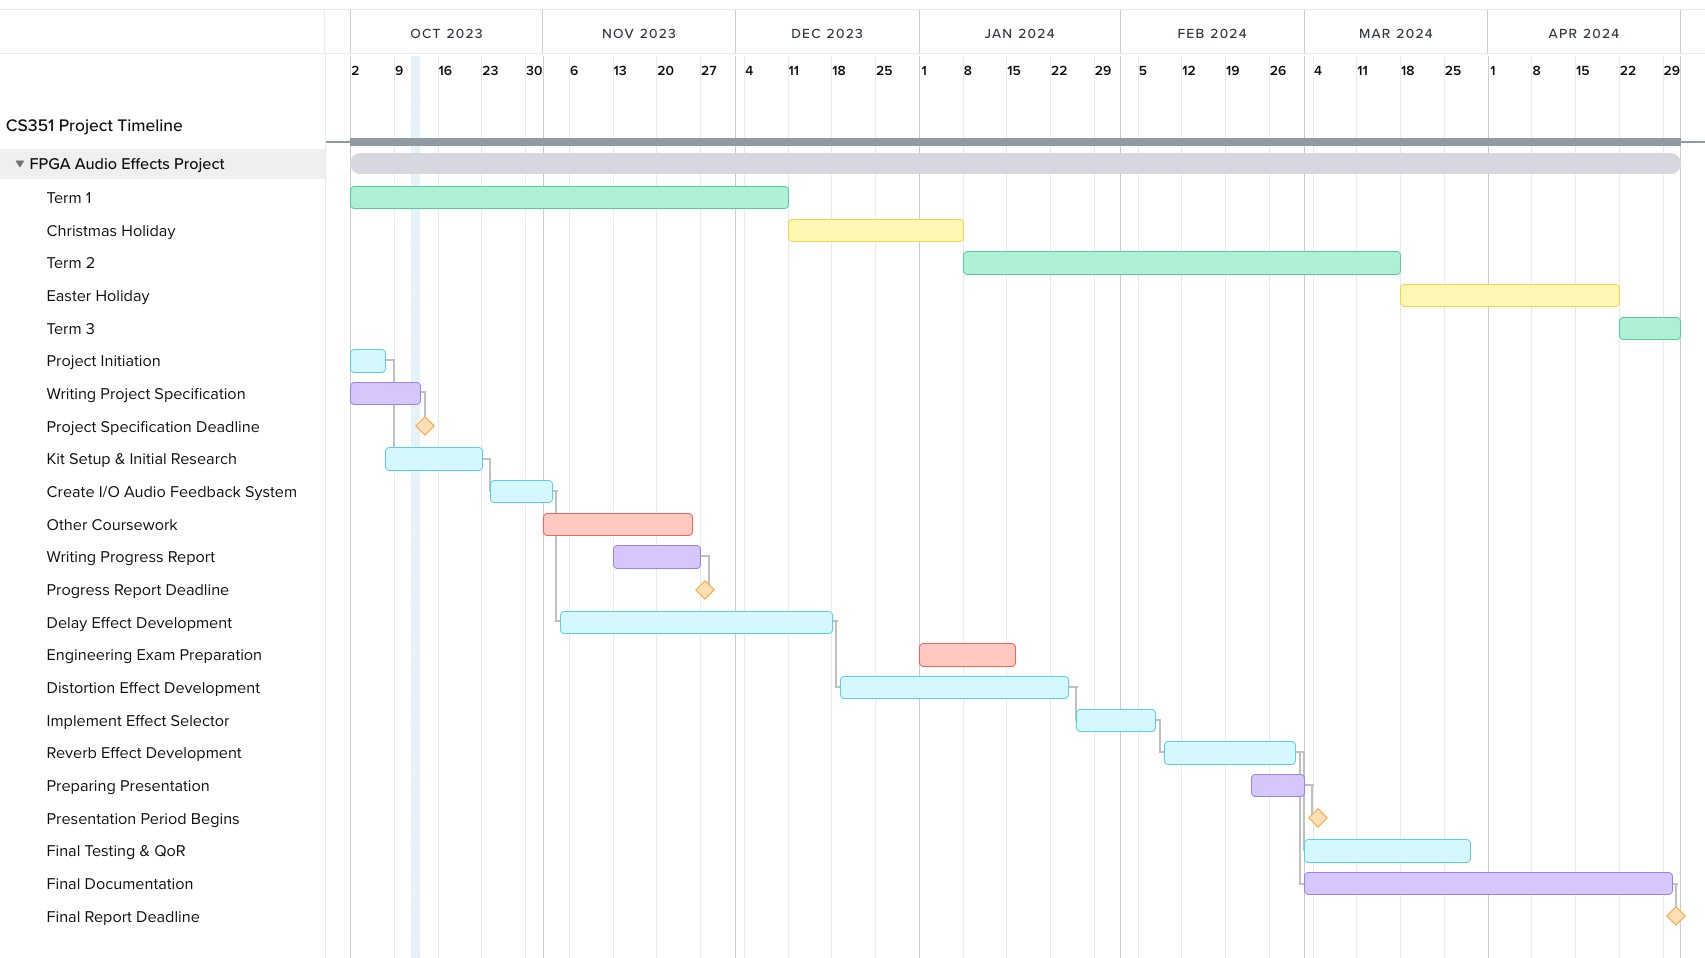
\includegraphics[width=1.0\textwidth]{specification/cs351-spec-gantt-chart2.jpeg}
\caption{Project tasks organised in a Gantt chart}
\end{figure}

The timetable includes events that might interfere with the evolution of the system, and tasks surrounding these events have been assigned longer durations.
